\documentclass[12pt,a4paper]{article}
\usepackage{cirilica}
\usepackage{multicol}
\usepackage{graphicx}
\usepackage{geometry}
\geometry{
left = 2cm,
right = 2cm,
top = 2cm,
bottom = 2cm
}

\title{\lat{Latex}}
\author{Ime i prezime}
\pagestyle{myheadings}

\markright{Primer dokumenta}
\begin{document}

\maketitle
\thispagestyle{empty}
\newpage
\section {Matematika}
\subsection{Furijeova analiza}
Svaka periodi\v cna funkcija\footnote{pogledati kako se defini\v se funkcija}, po teoriji Furijeovih redova, mo\v ze se predstaviti pomo\' cu beskona\v cno monogo ortogonalnih funkcija. Kako ovaj na\v cin predstavljanja funkcije pru\v za mogu\' cnost sasvim druga\v cije analize u odnosu na analizu u vremenskom domenu, postavlja se pitanje da li je mogu\' ce istu ideju pro\v siriti na funkcije koje nisu periodi\v cne. Ako se neperiodi\v cna funkcija posmatra kao periodi\v cna sa beskona\v cno velikim periodom, Furijeova transformacija pro\v siruje ovaj koncept razlaganja funkcija i na neperiodi\v cne funkcije.

\subsubsection{Formule}

\begin{enumerate}
  \item Period\v cne funkcije $f(x) = f(x +2 \pi )$
  \item Predstavljanje : $ a \cos \omega x + b \sin \omega x \quad a,b \in \mathbf{R}$
  \item $\prod_{i=N}^{N} = f(i)$
\end{enumerate}


\section{Modelovanje tema}

\begin{multicols}{2}
{\lat \textit{Latent Dirichlet Allocation}}, nadalje {\lat LDA}, je najjednostavniji pristup problemu modelovanja tema, i njegova primena je predmet ovog rada.
Osnovna karakteristika{\lat LDA } algoritma je mogu\' cnost \textbf{izdvajanja} tema koje su prisutne u nekoj kolekciji dokumenata bez bilo kakvog dodatnog znanja. Dakle, primenom {\lat LDA}-a mogu\' ce je otkriti teme "o kojima govori" zadati skup dokumenata a da se pritom nikakvo dodatno ekspertsko znanje ne uklju\v cuje.
Polazna pretpostavka{\lat LDA}-a je da svaki dokument u kolekciji dokumenata "govori o" vi\v se tema. Opravdanost ove pretpostavke bi\' ce ilustrovana na nekoliko primera.
Dobro je poznat roman Branka \' Copi\' ca "Orlovi rano lete". Ukoliko bi neko ko nije pro\v citao ovi knjigu \v zeleo da zna "o \v cemu se radi" u njoj, najverovatnije bi dobio odgovor da je u pitanju knjiga koja se bavi do\v zivljajima grupe de\v caka na po\v cetku Drugog svetskog rata. Iako je to naj\v siri okvir romana, u njemu su prisutne i teme o ljubavi, dru\v zenju, prijateljstvu, ratu, pustolovinama itd. Prema tome, roman, op\v ste gledano, obuhvata vi\v se tema, ali se sa nekoliko njih intenzivno bavi.
\end{multicols}
% \vspace{3cm}

\subsection{Grafi\v cki primer dokumenta}
Generalno, proces zaklju\v civanja tematike dokumenta mo\v ze se ilustrovati slede\' cim primerom.
Na Slici \ref{fig:tmSlika1} predstavljen je \v clanak {\lat \textit{Seeking Life's Bare(Genetic) Necessities}} koji govori o upotrebi analize podataka za određivanje broja gena koji organizam treba da poseduje da bi pre\v ziveo (u evolutivnom smislu). Mo\v ze se uo\v citi da su tri najzastupljenije oblasti u ovom tekstu - analiza podataka, evolutivna biologija i genetika. Na slici su ru\v cno ozna\v cene neke re\v ci koje pripadaju ovim oblastima. Re\v ci koje se mogu svrstati u oblast \textit{analize podataka} ozna\v cene su plavom bojom, re\v ci koje pripadaju \textit{genetici} ozna\v cene su \v zutom bojom, dok su re\v ci koje se odnose na \textit{evolutivnu biologiju} ozna\v cene roze bojom. Ukoliko bi se ova procedura primenila na svaku re\v c teksta, jasno bi se uo\v cilo koliko je koja tema zastupljena u ovom tekstu. Matemati\v cki, \textit{prisustvo} teme u tekstu se ozna\v cava odnosom broja re\v ci "obojenih" datom bojom i ukupnog broja re\v ci u tekstu.

\begin{figure}[h!]
    \centering
    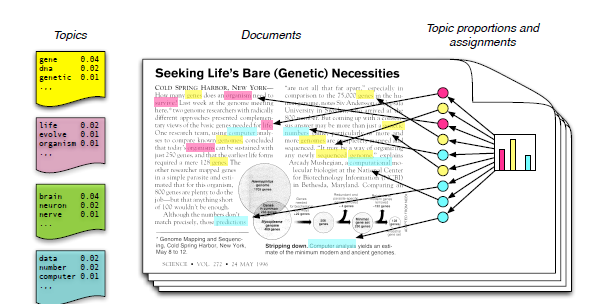
\includegraphics[scale=0.7]{tm.png}
	\caption{Primer \v clanka}
	\label{fig:tmSlika1}
\end{figure}


Naravno, postoje re\v ci koje se mogu svrstati u vi\v se od jedne teme. Takve re\v ci bi bile obojene sa dve ili vi\v se boja, ali zbog preglednosti slike, takvi slu\v cajevi su izostavljeni.
\newpage

\subsection{Prikaz rada algoritma}
Rad algoritama prikazanog na Slici \ref{fig:tmSlika1}  je slede\' ci
\begin{enumerate}
  \item Prvi korak :
  \begin{center}
    \begin{tabular}{|c|c|c|c|c|}
    \hline
    % after \\: \hline or \cline{col1-col2} \cline{col3-col4} ...
    \multicolumn{5}{|c|}{Primer dokumenta} \\ \hline
      &   &   &   &   \\ \hline
    matematika & fizika & hemija & biologija & istorija \\
    \hline
  \end{tabular}
  \end{center}

  \item
   Drugi korak :
   \begin{center}
     \begin{tabular}{|c|c|c|c|c|}
    \hline
    % after \\: \hline or \cline{col1-col2} \cline{col3-col4} ...
    \multicolumn{5}{|c|}{Primer dokumenta} \\ \hline
    $\sum_{1}^{N} f(reci)$  & $\sum_{1}^{N} f(reci)$   &  $\sum_{1}^{N} f(reci)$  &  $\sum_{1}^{N} f(reci)$  &  $\sum_{1}^{N} f(reci)$  \\ \hline
    matematika & fizika & hemija & biologija & istorija \\
    \hline
  \end{tabular}
   \end{center}
  \item Finalni korak :
  \begin{center}
     \begin{tabular}{|l|c|c|c|}
    \hline
    % after \\: \hline or \cline{col1-col2} \cline{col3-col4} ...
    Re\v ci & \multicolumn{3}{c|}{Teme} \\ \hline \hline
      & 1 & 2 & 3 \\ \hline
    matematika & $n_1^1$ & $n_2^1$ & $n_3^1$ \\ \hline
    fizika &  $n_1^2$ & $n_2^2$ & $n_3^2$\\ \hline
    hemija &  $n_1^3$ & $n_2^3$ & $n_3^3$ \\ \hline
    biologija & $n_1^4$ & $n_2^4$ & $n_3^4$ \\ \hline
    istorija & $n_1^5$ & $n_2^5$ & $n_3^5$ \\ \hline
    \hline
  \end{tabular}

  \end{center}

\end{enumerate}

\begin{thebibliography}{99}
\bibitem{mell} {\lat Mell, Peter, and Tim Grance. The NIST definition of cloud computing. (2011).}
\bibitem{buyya} {\lat Buyya, Rajkumar, et al. "Cloud computing and emerging IT platforms: Vision, hype, and reality for delivering computing as the 5th utility." Future Generation computer systems 25.6 (2009): 599-616.}
\end{thebibliography}


\newpage
\tableofcontents
\thispagestyle{empty}
\end{document} 